\documentclass[a4paper]{article}
\usepackage[a4paper, portrait, margin=1cm, bottom=2cm]{geometry}
\usepackage{amsmath}
\usepackage{mathtools}
\usepackage{fontspec}
\usepackage{graphicx}
\usepackage{indentfirst}

\setmainfont[Ligatures=TeX]{Linux Libertine}
\graphicspath{./graphics/}

\title{Информационные технологии. Лекция 12. Функциональная безопасность}
\author{Студент группы 2305 Макурин Александр}
\date{22 мая 2023}

\renewcommand{\labelenumii}{\theenumii}
\renewcommand{\theenumii}{\arabic{enumii}.}
\setlength{\leftmarginii}{1.8ex}

\begin{document}
\maketitle

Виды проблем (сбоев) в ИБ:
\begin{itemize}
    \item сбой
    \item отказ
    \item нарушение
\end{itemize}

Места сбоев:
\begin{itemize}
    \item органы управления
    \item датчики
    \item переход от СУ к ОУ
\end{itemize}

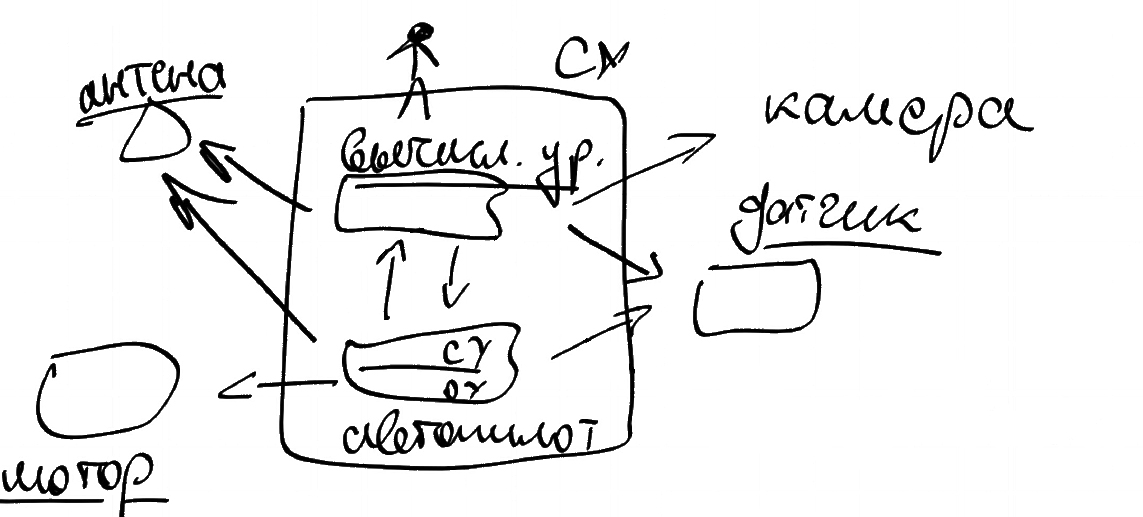
\includegraphics[width=0.8\textwidth]{graphics/pic00.jpg}

$S^{t + 1} = S^t + U^*$, где $U^*$ — реально полученное управляющее воздействие.

$U^* = f(K_PP +K_VV) + U$. $K_{P,V}$ — передаточные коэффициенты. $U$ — то, что хотим сделать (запланированное воздействие). $P$ — погрешность анализа. $V$ — «словарь», обычно неизменный (const). $f(...)$ — поправки.

Проблема — в данной формуле не заложена возможность сбоя.

На примере датчиков:
\begin{itemize}
    \item $\overline{P} = AP$ — сбой. $A$ — случайный ряд.
    \item $\overline{P} = \text{const}$ — отказ.
    \item $\overline{P} = AP + l$ — нарушение. $l$ — смещение.
\end{itemize}

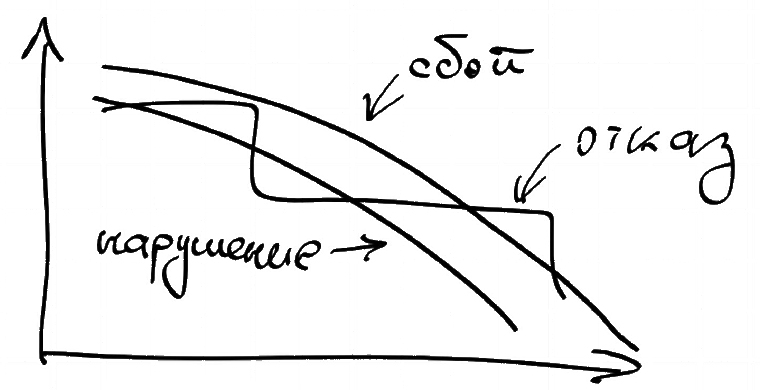
\includegraphics[width=0.5\textwidth]{graphics/pic01.jpg}

$U^* = G(K_PP + K_VV) + U$

$G = \begin{cases}I \\ diag(0_i)\end{cases}$ — если элемент функционирует неверно, то соответствующий элементы диагональной матриц равен $0$.

Когда элемент $j$ вышел из строя, его состояние неизвестно и требуется вносить поправку в управляющее воздействие с учётом этого: $\overline{U} = U^* + \Delta U_j$.

Порядок действий при взаимодействии с отказом (сбоем/отказом/нарушением):
\begin{enumerate}
    \item Обнаружить отказ и зафиксировать время обнаружения и предыдущее состояние системы ($t_\text{обн}$ и $U_{t_\text{обн} - 1}$).
    \item Локализовать отказавший элемент $j$.
    \item Противодействовать отказу коменсацией управляющего воздействия $\Delta U_j = U_{t_\text{обн}} - U_{t_0}$.
\end{enumerate}

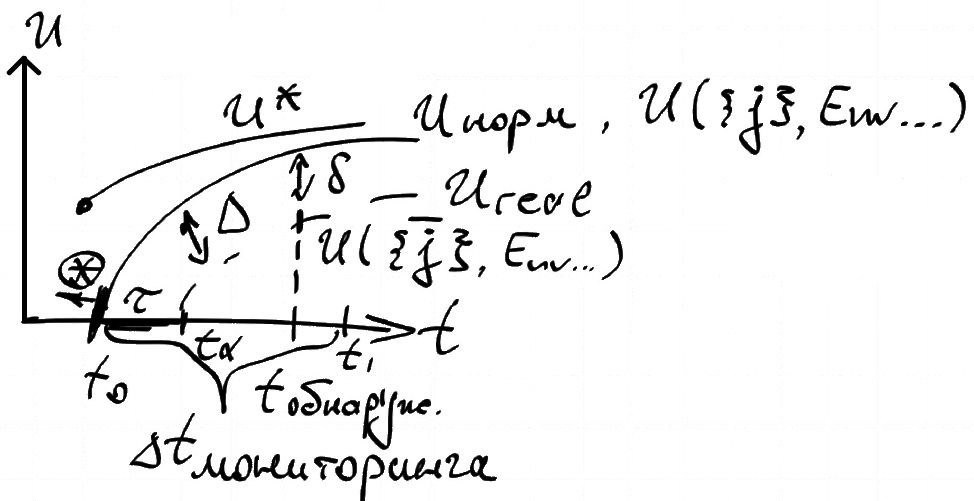
\includegraphics[width=0.5\textwidth]{graphics/pic02.jpg}

$|\{j\}| > |\{\overline{j}\}|$

$\tau$ — разница между тем, что должно было быть и тем, что есть.

$S^{t_0} = S^{t_{0-1}} + K_P^\text{Камер}P_\text{Камер} + K_P^\text{Сенсоров}P_\text{Сенсоров} + K_VV + U$

$S^{t_1 - \delta} = S^{t_0} + K_P^\text{л}P_U + U$

$S^{t-1} = S^{t_0} + K_P^\text{л}P_U + K_P^\text{Сенсоров}P_\text{Сенсоров} + U$

$K_r = \dfrac{\delta U(t_0, t_1, \dfrac{\delta U(t_0)}{\delta U_j})}{\delta U_j}$. $\dfrac{\delta U(t_0)}{\delta U_j}$ — коэффициент чувствительности (чем он выше, тем важнее датчик).

$U(t_0, t_1, \Delta U) = K_r \cdot \Delta U_j(t_\alpha)$. $\Delta U = \begin{cases}
        0 \text{ — сенсор был не нужен}   \\
        \alpha \text{ — сенсор был нужен} \\
    \end{cases}$ — коррекция.

Если на участке времени сенсор был не нужен, то его можно не корректировать на этом учатке.
\begin{enumerate}
    \item $t_\text{поиска}$ $|\text{Гипотеза}| = |\{j\}|$ — строим графики гипотез для $U_{\text{реал}_j}$.
    \item \begin{enumerate}
              \item $\tau_\alpha = \arg \min \phi_j(\tau)$ \\
                    $\phi = \arccos \dfrac{\Delta U \dfrac{\delta U}{\delta U_j}}{||\Delta U|| \left|\left|\dfrac{\delta U}{\delta U_j}\right|\right|}$ \\
                    $\phi_j(\tau) \leq \overline{\phi_j}$ — порог, который мы назначим
              \item $j^* = \arg \min \phi(\tau_j)$ \\
                    $\Delta U_j = \dfrac{\delta U}{\delta U_j} \cdot \Delta U$ \\
                    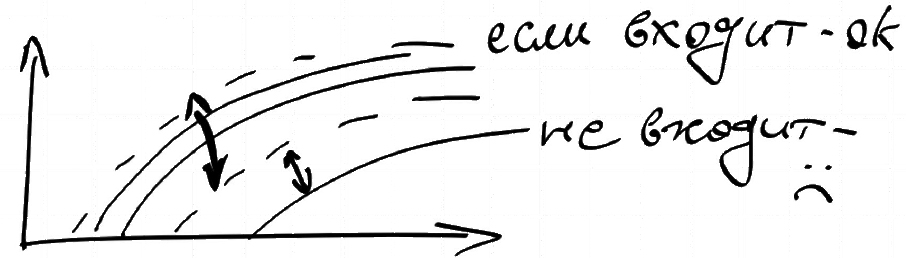
\includegraphics[width=0.3\textwidth]{graphics/pic03.jpg}
          \end{enumerate}
\end{enumerate}

Тоже самое повторяем для $K_P, K_V$ и $P$.
\end{document}